% Four alternatives are drawn about their own local origins on a common baseline.
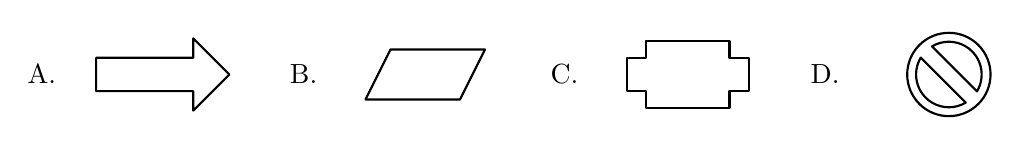
\begin{tikzpicture}[x=1bp,y=1bp,line width=.78bp,line cap=round,line join=round,
  option/.style={font=\fontsize{10.4bp}{12bp}\selectfont,anchor=east,inner sep=0pt}]
  \foreach \x/\choice in {0/A,94/B,188/C,282/D}
    \node[option] at (\x+10,0) {\choice.};
  \begin{scope}[shift={(49,0)}]
    \draw (-25,-6) -- (10,-6) -- (10,-13) -- (23,0) --
           (10,13) -- (10,6) -- (-25,6) -- cycle;
  \end{scope}
  \begin{scope}[shift={(143,0)}]
    \draw (-22,-9) -- (12,-9) -- (21,9) -- (-13,9) -- cycle;
  \end{scope}
  \begin{scope}[shift={(237,0)}]
    \draw (-15,12) -- (15,12) -- (15,6) -- (22,6) -- (22,-6) --
           (15,-6) -- (15,-12) -- (-15,-12) -- (-15,-6) --
           (-22,-6) -- (-22,6) -- (-15,6) -- cycle;
  \end{scope}
  \begin{scope}[shift={(331,0)},rotate=-45]
    \draw (0,0) circle[radius=15bp];
    % Two equal circular segments leave the white diagonal stroke unfilled.
    \draw (14:11.8) arc[start angle=14,end angle=166,radius=11.8bp] -- cycle;
    \draw (194:11.8) arc[start angle=194,end angle=346,radius=11.8bp] -- cycle;
  \end{scope}
\end{tikzpicture}
